\documentclass{article}[12 pt]
\usepackage{amssymb}
\usepackage{amsthm}
\usepackage{amsmath}
\usepackage{appendix}
\usepackage{array}
\usepackage{geometry}
\usepackage{enumitem}
\usepackage{graphicx}
\usepackage{subfig}
\usepackage{caption}
\usepackage{url}
\usepackage{float}
\usepackage{pdfpages}
\usepackage{shortvrb}
\usepackage{mathtools}
\usepackage{multirow}
\usepackage{hyperref}
\usepackage{algorithm}
\usepackage[noend]{algpseudocode}
\usepackage{bm}

\def\BibTeX{{\rm B\kern-.05em{\sc i\kern-.025em b}\kern-.08em
		T\kern-.1667em\lower.7ex\hbox{E}\kern-.125emX}}
\graphicspath{{"C:/Users/Conma/Documents/ImageProcessing/HW04/Report/Images/"}}
% \graphicspath{{"//ece-azare-nas1.ad.ufl.edu/ece-azare-nas/Profile/cmccurley/Desktop/ImageProcessing/HW04/Report/Images/"}}
\geometry{margin=1 in}

\newcommand{\smallvskip}{\vspace{5 pt}}
\newcommand{\medvskip}{\vspace{50 pt}}
\newcommand{\bigvskip}{\vspace{100 pt}}
\newcommand{\tR}{\mathtt{R}}

%===================================================================================================================
\begin{document}
	
\begin{center}
	\textbf{\Large Connor McCurley} \\
	EEE 6512 \qquad \textbf{\large Homework 4 Due October 13, 2018} \qquad Fall 2018 
\end{center}

%===================================================================================================================
\section*{Part I Questions}

\begin{enumerate}
\item As seen below, the first component is worked by hand, while the rest were computed through Matlab.

\begin{figure}[H]
\captionsetup[subfloat]{labelformat=empty}
\centering
\subfloat[]{
  \includegraphics[width=105mm]{"DFT"}
}
\newline
\subfloat[]{
  \includegraphics[width=105mm]{"FFT"}
}
\caption{Left: First two components of the DFT computed by hand Right: Matlab Solution}
\end{figure}

% \newpage
\item Transforming the matrix results in the following:

\begin{figure}[H]
\captionsetup[subfloat]{labelformat=empty}
\centering
\subfloat[]{
  \includegraphics[width=65mm]{"AltDFT"}
}
\newline
\subfloat[]{
  \includegraphics[width=105mm]{"AlternateFFT"}
}
\caption{Top: Image transformed by $(-1)^{x+y}$ Bottom: DFT solution provided by Matlab}
\end{figure}

The computation of the DFT was provided by Matlab's fft2() function.

\item As seen by the final solutions, the resulting DFTs are just shifted versions of each other.  The matrix transformed by the (-1) term shifts the frequencies so that the DC is centered and the other frequencies expand radially from there.

\item Question 7.25:
	\begin{enumerate}[label=\alph*]
		\item In the HSI space, each pure color region demonstrates a Saturation of 1 and an Intensity of 1/3 (given by equations 7-18 and 7-19 in the textbook).  However, each converted color demonstrates a different hue, the R at 0, G at $\frac{1}{3}$ and B at $\frac{2}{3}$, which are the normalized hue values given by equations 7-17 and 7-17 in the textbook.

		\item Smoothing the resulting HSI image over the saturation component will not affect the image visually, the only would be in intensity. 

		\item If smoothing is applied in just the hue channel would not be altered by a kernel smoothing.  Only intensity would be affected.
	\end{enumerate}

\end{enumerate}

\section*{Part II MATLAB Programming}
\begin{enumerate}
\item This question asked to identify and remove an anomalous frequency in a corrupted image.  This was done by observing the DFT of the image and multiplying the frequency image by a gaussian kernel to effectively smooth the high frequency components.  The bandwidth was chosen subjectively.  The image was then reconstructed using the inverse DFT.  While this method was adequate in removing the frequency interference, it resulted in loss of high frequency detail in the spatial domain.

\begin{center}
	\begin{figure}[H]
		\centering
		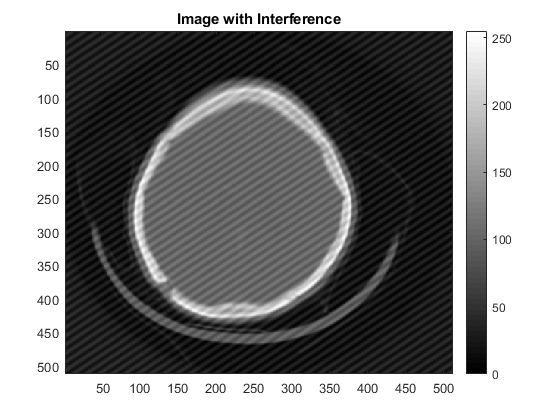
\includegraphics[width = 0.5\textwidth]{Images/interference.png}
		\caption{8-bit intensity image corrupted by frequency noise}
		\label{interference}
	\end{figure}
\end{center}
\begin{center}
	\begin{figure}[H]
		\centering
		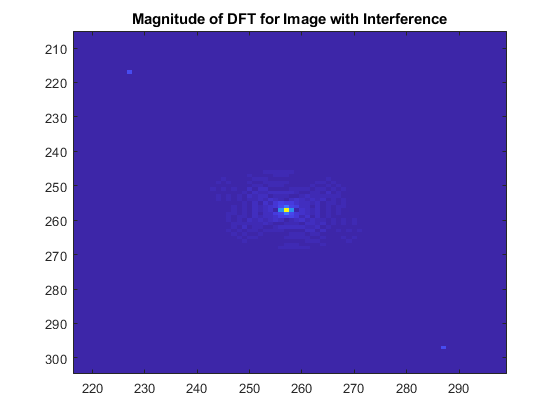
\includegraphics[width = 0.5\textwidth]{Images/dftNoisy.png}
		\caption{Zoomed in DFT of the corrupted image.  Anomalous frequencies can be seen in the corners of the zoomed image.}
		\label{dftNoisy}
	\end{figure}
\end{center}
\begin{center}
	\begin{figure}[H]
		\centering
		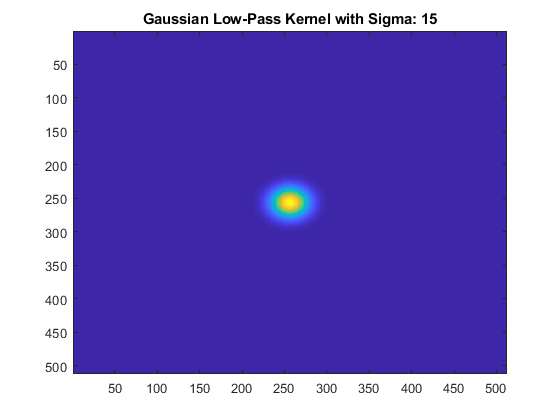
\includegraphics[width = 0.5\textwidth]{Images/kernel.png}
		\caption{Gaussian kernel with bandwidth $\sigma = 15$}
		\label{kernel}
	\end{figure}
\end{center}
\begin{center}
	\begin{figure}[H]
		\centering
		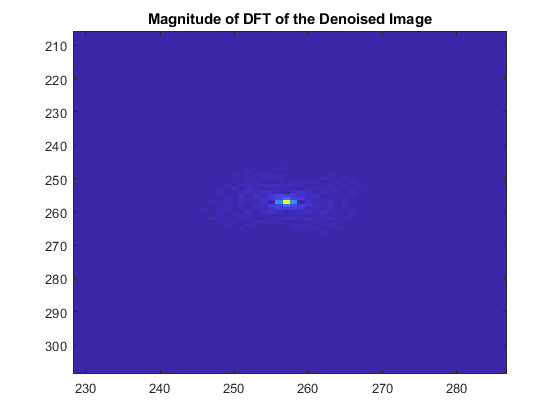
\includegraphics[width = 0.5\textwidth]{Images/dftClean.png}
		\caption{"Cleaned" dft image zoomed in.  This image is a result of the multiplication of the gaussian kernel and corrupted dft image.  It can be observed that the anomalous frequencies seen in fig \ref{dftNoisy} have been attenuated.}
		\label{dftClean}
	\end{figure}
\end{center}
\begin{center}
	\begin{figure}[H]
		\centering
		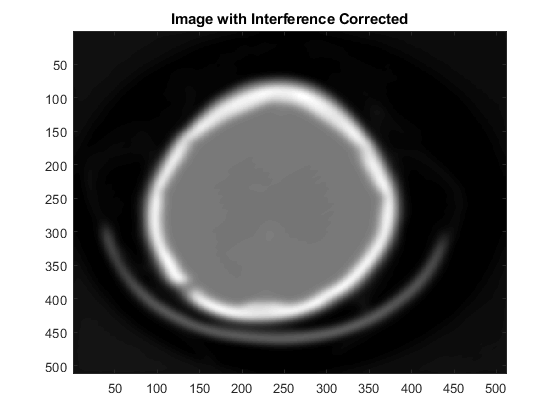
\includegraphics[width = 0.5\textwidth]{Images/denoised.png}
		\caption{Filtered image of fig \ref{interference}.  Smoothing was performed in the frequency domain.}
		\label{denoised}
	\end{figure}
\end{center}

\item This question asked to convert the gray-scale images from homework 2 into 8-color pseudo-color images with the colors: red, blue, green, yellow, orange, purple, brown, and black.  Results of the conversion using intensity slicing are presented below.

\begin{figure}[H]
\captionsetup[subfloat]{labelformat=empty}
\centering
\subfloat[]{
  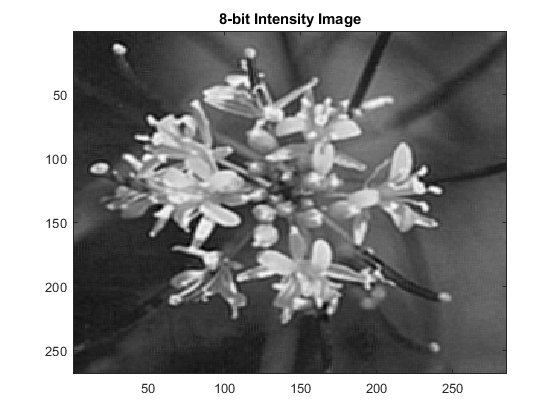
\includegraphics[width=70mm]{flowers.png}
}
\subfloat[]{
  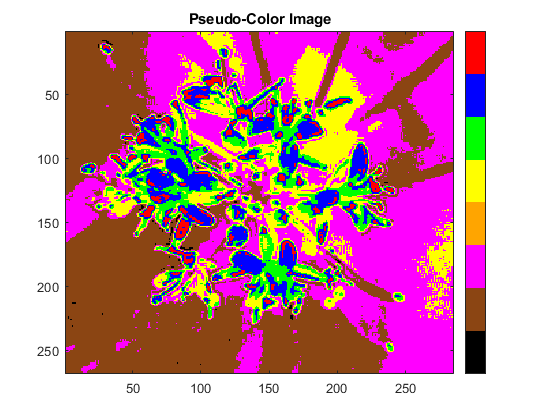
\includegraphics[width=70mm]{pcFlowers.png}
}
\hspace{0mm}
\subfloat[]{
  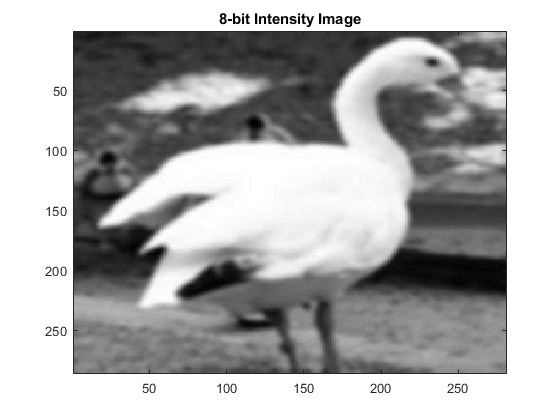
\includegraphics[width=70mm]{swan.png}
}
\subfloat[]{
  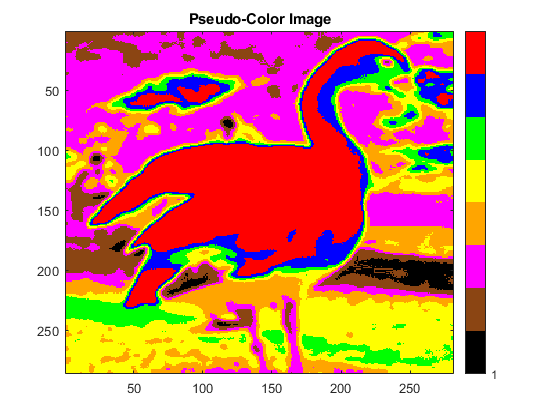
\includegraphics[width=70mm]{pcSwan.png}
}
\hspace{0mm}
\subfloat[]{
  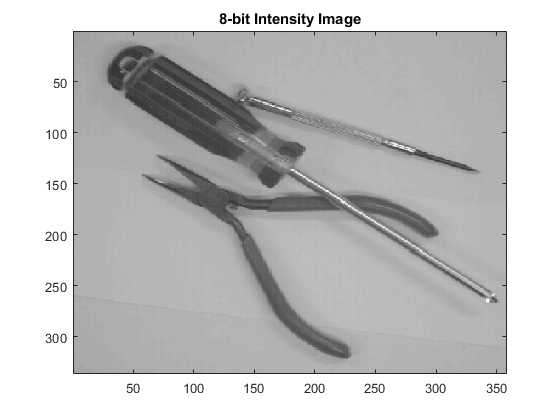
\includegraphics[width=70mm]{tools.png}
}
\subfloat[]{
  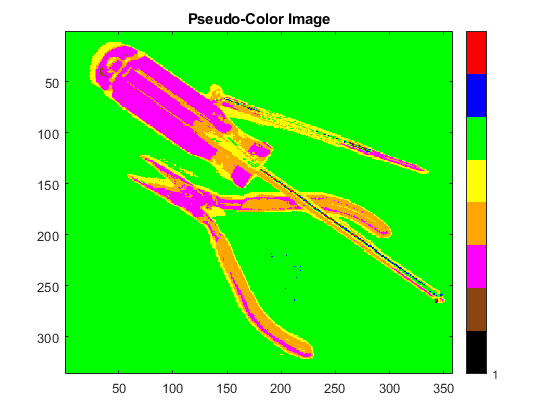
\includegraphics[width=70mm]{pcTools.png}
}
\caption{Left Column: 8-bit intensity images Right Column: Corresponding 8-color pseudo images}
\label{pc}
\end{figure}

My code generated the pseudo-color images by first creating a look-up table of  integer values.  The table contained 8 rows  representing the 8 color bins.  Each row contained 32 sequential integer values.  For example, the first row contained integers 0:31, the second row 32:63, and so on.  Each element of the gray-scale image was compared to the look-up table and a label was provided as the corresponding row in the table.   This effectively binned all 256 gray-scale values into the 8 color bins.  A single color was applied to each bin to get a pseudo-color image.
\end{enumerate}

\section*{Part III Extra Credit}
For this portion of the assignment, my code converted the scene provided into  3 separate images of colorspace RGB, HSI, and LAB, respectively. Each image was then segmented using color slicing.  Prototype regions were selected from areas of each image to include sky, cloud, water, sand, rock, and vegetation.  Each prototye region was averaged to provide a single feature vector prototype.  Euclidean distance was calculated between each pixel in an image and the set of prototypes.  The pixel was assigned the label of the closest prototype.  This process was repeated for the RGB, HSI, and LAB color spaces.

\begin{figure}[H]
\captionsetup[subfloat]{labelformat=empty}
\centering
\subfloat[]{
  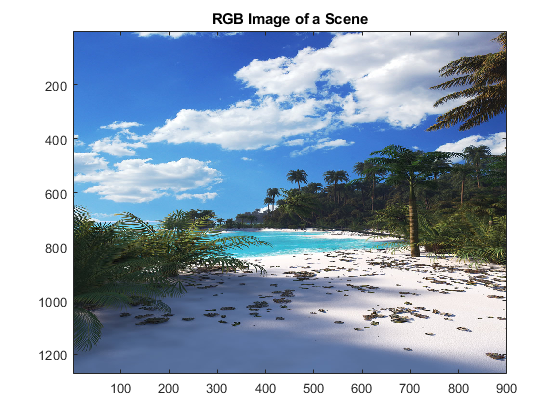
\includegraphics[width=40mm]{rgbScene.png}
}
\subfloat[]{
  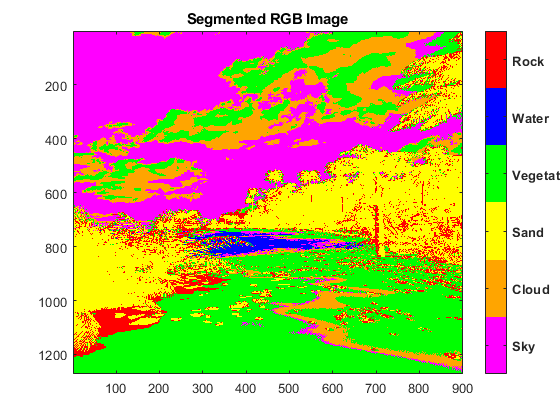
\includegraphics[width=70mm]{segmentedRGB.png}
}
\hspace{0mm}
\subfloat[]{
  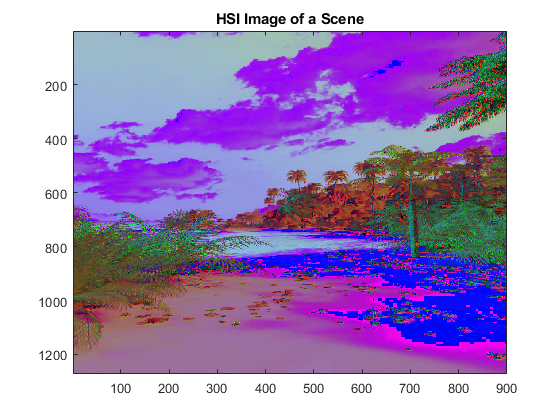
\includegraphics[width=40mm]{hsiScene.png}
}
\subfloat[]{
  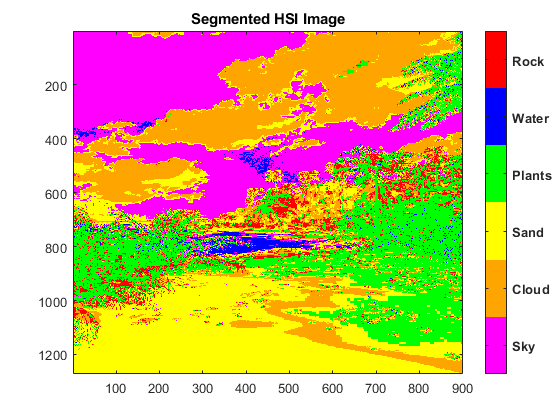
\includegraphics[width=70mm]{segmentedHSI.png}
}
\hspace{0mm}
\subfloat[]{
  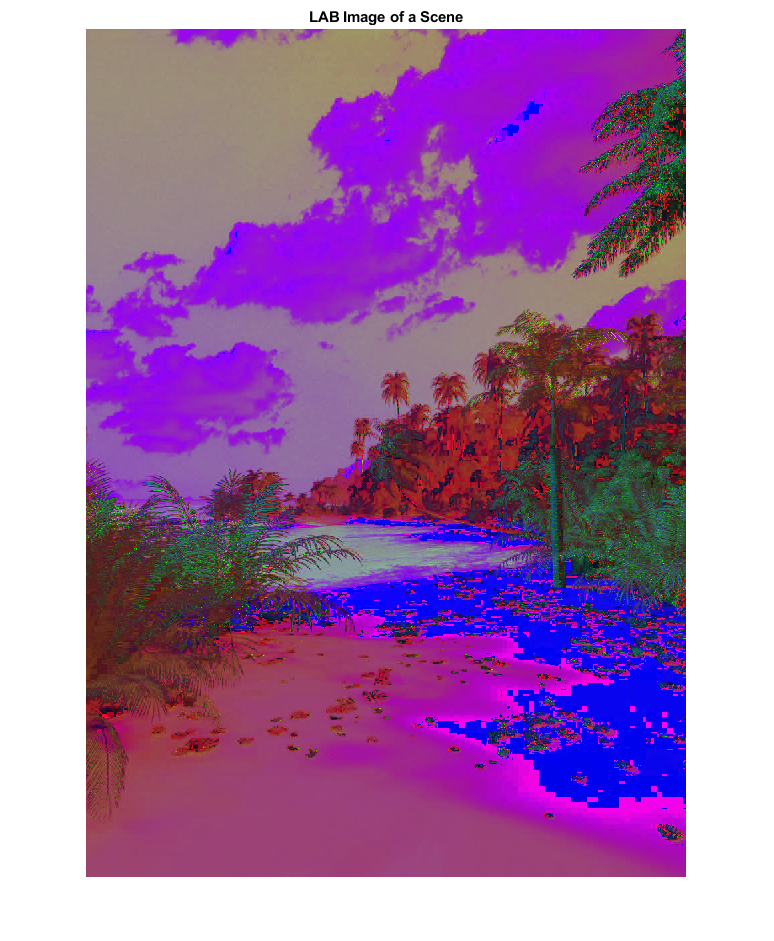
\includegraphics[width=40mm]{labScene.png}
}
\subfloat[]{
  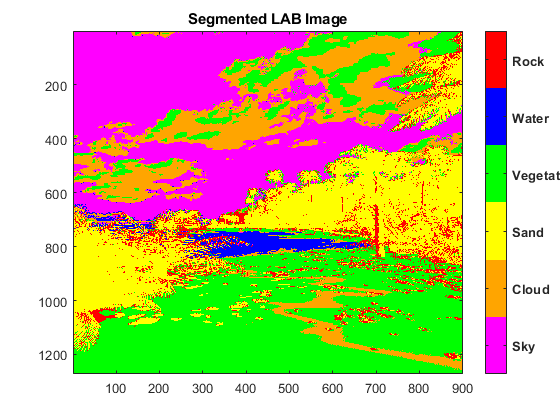
\includegraphics[width=70mm]{segmentedLAB.png}
}
\caption{Left Column: Original in rgb,hsi, and lab color spaces from top to bottom, respectively.  Right column: Corresponding segmented image}
\label{pc}
\end{figure}

It is worth noting that th

 \noindent 
 Accompanying code is provided in $mccurleyHW04.m$, $removeInterference.m$, $pseudoColor.m$, and $colorSegmentation.m$


\end{document}
